\section{Method}

\begin{figure}[t]
    \centering
    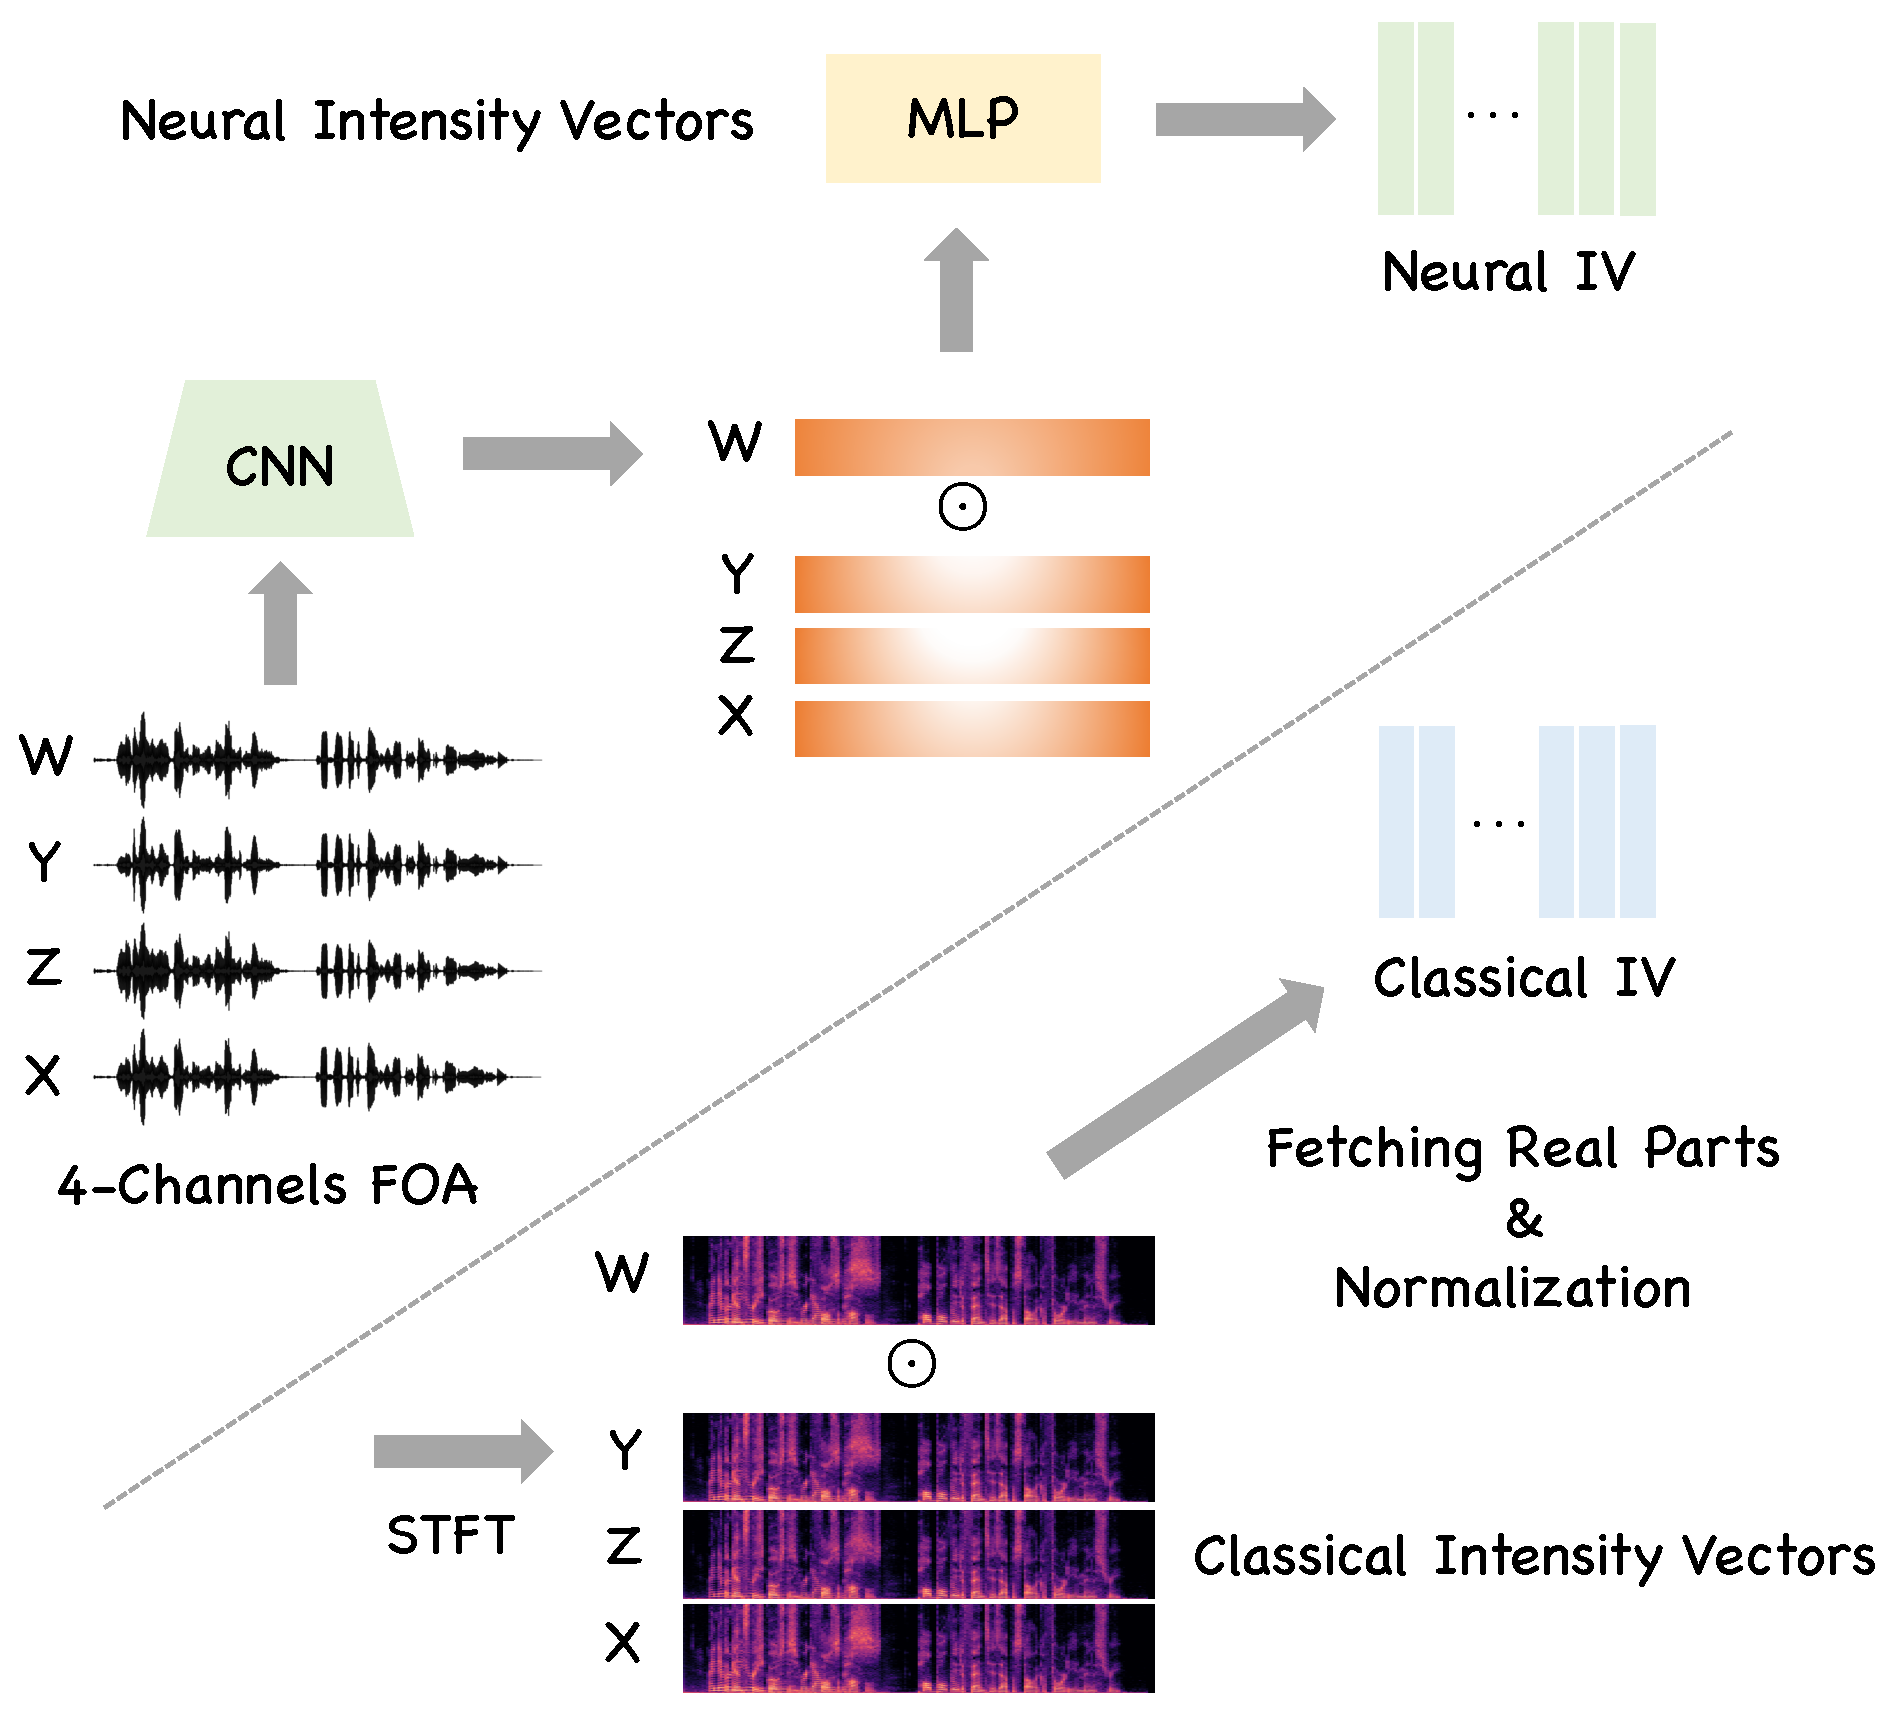
\includegraphics[width=1.0\linewidth]{IV-2.pdf}
    \caption{Comparisons between Classical IV and Neural IV.}
    \label{fig:neural_iv}
\end{figure}

\subsection{Intensity Vector for Audio Localization}

We extract spatial cues from FOA using the intensity vector (Classical IV) \cite{yasuda2020sound}. 
Following \cite{tang2024can}, we compute Classical IV features and use them to augment semantic audio representations with directional information.
%
Let $F_W$ denote the complex spectrogram of the omnidirectional FOA channel $W$, and let $F_C$ denote the complex spectrogram of the directional channels $C \in \{X, Y, Z\}$. 
The cross-spectrum for each axis is obtained as:
\begin{equation}
    I'_C = F_W^* \odot F_C,
\end{equation}
where $\odot$ denotes the Hadamard product and $F_W^*$ is the complex conjugate of $F_W$. 
The active intensity feature is then constructed by concatenating the real parts:
\begin{equation}
    \mathbf{I} = \operatorname{Concat}_{C \in \{X,Y,Z\}} \left( \mathcal{R}(I'_C) \right),
\end{equation}
Finally, we apply $L_2$-normalized $\mathbf{I} / \|\mathbf{I}\|_2$ to ensure numerical stability during training.

\subsection{Neural Intensity Vector}
Classical IV rely on fixed STFT-based signal processing, which often produces suboptimal representations in highly reverberant or overlapping-source environments. To address this limitation, here we introduce the Neural IV, a data-driven spatial encoder that learns to extract robust geometric cues directly from raw FOA waveforms.

As shown in Fig. \ref{fig:neural_iv}, Neural IV replaces the STFT transformation with a learnable CNN backbone. We adopt the data2vec \cite{baevski2022data2vec} frontend to ensure 50Hz frame rate, utilizing a 7-layer 1D-CNN with kernel sizes of $(10, 3, 3, 3, 3, 2, 2)$ and strides of $(5, 2, 2, 2, 2, 2, 2)$.
%
Let $f_W$ and $f_C$ denote the CNN-encoded latent features corresponding to the omnidirectional and directional channels ($C \in \{X, Y, Z\}$), respectively.
We generalize the physical principle of acoustic intensity to the latent space by computing the element-wise product of the omnidirectional ($f_W$) and directional ($f_C$) features:
\begin{equation}
    h_C = f_W \odot f_C, \quad \text{where } C \in \{X, Y, Z\}.
\end{equation}
%
These interaction features are then concatenated to form a unified spatial representation $\mathbf{H}'$:
\begin{equation}
    \mathbf{H}' = \operatorname{Concat}(h_X, h_Y, h_Z).
\end{equation}
%
Finally, we use a multilayer perceptron (MLP) to project these features into the final robust spatial embedding $\mathbf{v}_\text{NIV}$:
\begin{equation}
    \mathbf{v}_\text{NIV} = \operatorname{Linear}(\operatorname{ReLU}(\operatorname{Linear}(\mathbf{H}'))).
\end{equation}

\begin{figure*}[t] 
    \centering
    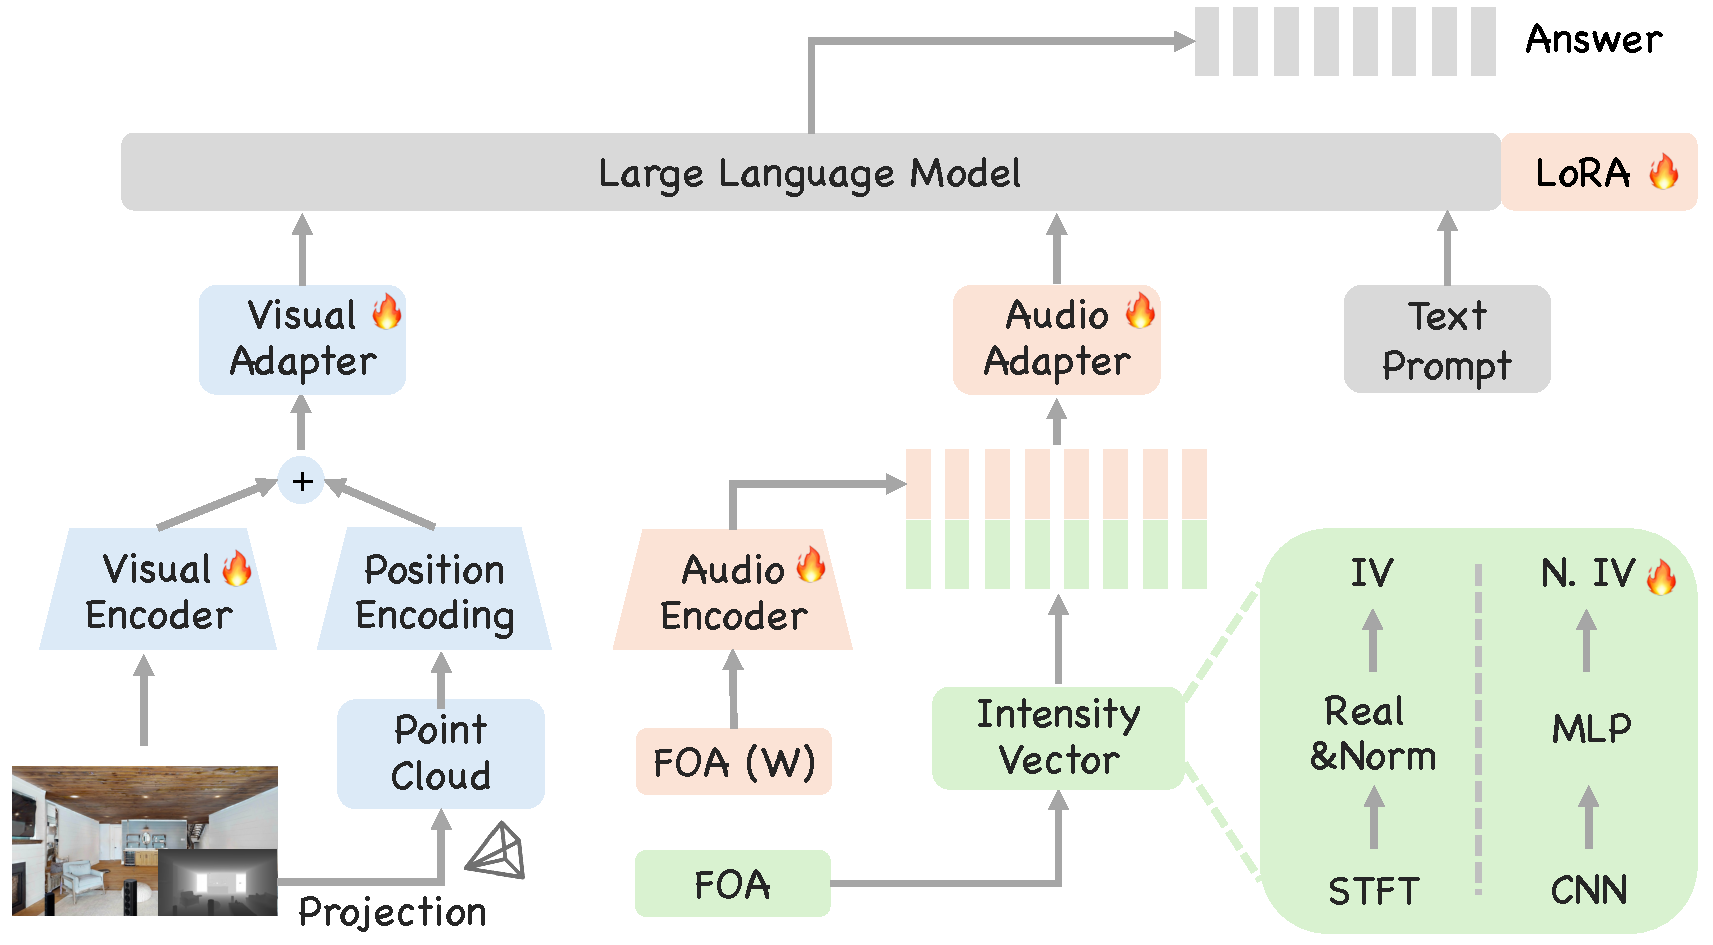
\includegraphics[width=0.85\linewidth]{architecture-2.pdf}
\caption{\textbf{Overview of the JAEGER Architecture.} The framework processes RGB-D and FOA inputs. 
\textbf{(1) Visual Stream:} RGB features are fused with 3D-aware positional encodings derived from depth-projected Point Clouds. 
\textbf{(2) Audio Stream:} Semantic features are extracted from the omnidirectional channel (FOA W). For spatial cues, we compare Classical IV with Neural IV (N. IV). Specifically, IV derives features via STFT followed by fetching real parts and normalization, whereas Neural IV extracts geometric features from raw waveforms using channel-wise 1D-CNNs followed by an MLP.}
    \label{fig:architecture}
\end{figure*}

\subsection{3D-aware Visual Encoding}

To empower the visual encoder with 3D awareness, we employ a widely used depth embedding strategy \cite{zheng2025video, wang2025n3d}. Specifically, we inject sinusoidal encodings of downsampled metric coordinates into the visual embeddings.

\textbf{Metric Point Cloud Reconstruction.}
Given an RGB image $I \in \mathbb{R}^{H \times W \times 3}$ and its aligned depth map $D \in \mathbb{R}^{H \times W}$, we reconstruct the metric point cloud $P \in \mathbb{R}^{H \times W \times 3}$. For each pixel location $(u, v)$ with depth value $D_{uv}$, the corresponding 3D coordinate $P_{uv}$ is obtained via back-projection:
\begin{equation}
    P_{uv} =  D_{uv} \cdot \begin{bmatrix} f_x & 0 & c_x \\ 0 & f_y & c_y \\ 0 & 0 & 1 \end{bmatrix}^{-1} \begin{bmatrix} u \\ v \\ 1 \end{bmatrix},
\end{equation}
where $(u, v)$ denotes the 2D pixel coordinates, and $f_x, f_y$ and $(c_x, c_y)$ represent the camera's focal lengths and principal point, respectively.

\textbf{3D-aware Positional Encoding.}
We align the dense geometry $P \in \mathbb{R}^{H \times W \times 3}$ with the spatial resolution of visual features $F_\text{visual} \in \mathbb{R}^{h \times w \times c}$ via adaptive average pooling. Each coordinate component $\alpha \in \{x, y, z\}$ of the aligned geometry is mapped to $\lfloor \frac{c}{3} \rfloor$ channels by sinusoidal functions:
\begin{equation}
    \begin{aligned}
        \text{PE}(\alpha, 2j) &= \sin\left( \frac{\alpha}{10000^{2j / \lfloor \frac{c}{3} \rfloor}} \right), \\
        \text{PE}(\alpha, 2j+1) &= \cos\left( \frac{\alpha}{10000^{2j / \lfloor \frac{c}{3} \rfloor}} \right),
    \end{aligned}
\end{equation}
for $j = 0, 1, \dots, \lfloor \frac{c}{6} \rfloor - 1$. The embeddings for the three axes are concatenated to form $F_{3D} \in \mathbb{R}^{h \times w \times c}$, which is then fused with the visual features via element-wise addition:
\begin{equation}
    \tilde{F}_\text{visual} = F_\text{visual} + F_\text{3D}.
\end{equation}

\subsection{Overall Model Architecture}

As shown in Figure \ref{fig:architecture}, JAEGER unifies multi-modal perception and reasoning through the following core modules:

\textbf{Visual Stream.} We fuse RGB semantic tokens with geometric priors derived from our 3D-aware Positional Encoding to explicitly ground visual representations in metric space.

\textbf{Audio Stream.} We adopt a dual-path design, extracting semantic content from the omnidirectional channel while capturing spatial cues via either \textit{Classical IV} or \textit{Neural IV}.

\textbf{LLM Backbone.} All multi-modal features are aligned via MLP adapters and fed into the LLM. We employ LoRA \cite{hu2022lora} to efficiently fine-tune the model for joint 3D grounding and reasoning.

\begin{table*}[t]
    \centering
    \setlength{\tabcolsep}{3pt} 
    \caption{Main results compared with baselines. \textbf{Task Definitions \& Metrics:} 
(1) \textbf{Audio DoA}: Detection of sound source arrival direction. Metric: Median Angular Error (MAE) in degrees ($^\circ$). 
(2) \textbf{Overlap Audio DoA}: MAE of a specific audio source's arrival angle when two audio clips overlap. 
(3) \textbf{3D IoU}: Mean Intersection over Union of the predicted 3D bounding box.
(4) \textbf{Visual Offset}:  Median distance deviation of the predicted object center coordinates from the ground truth. 
(5) \textbf{Reasoning 1-speaker}: Localizing one of multiple visible loudspeakers in the scene based on spatial audio cues from a single speaker. 
(6) \textbf{Reasoning 2-speaker}: Identifying a specific loudspeaker among multiple candidates based on the spatial location cues of a target speech in a two-speaker scenario. 
Reasoning tasks are evaluated by \textbf{Accuracy}. ``--'' indicates the model is incapable of performing the task.}
    \vspace{0.1in}
    
        \footnotesize
    \begin{tabular}{l c cccc cc}

    \toprule
    \multirow{2}{*}{Model} & \multirow{2}{*}{Modality} & \multicolumn{4}{c}{Perception} & \multicolumn{2}{c}{Reasoning} \\
    \cmidrule(lr){3-6} \cmidrule(lr){7-8}
    & & Audio DoA $\downarrow$ & Overlap DoA $\downarrow$ & 3D IoU $\uparrow$ & Visual Offset $\downarrow$ & 1-speaker $\uparrow$ & 2-speaker $\uparrow$ \\
    \midrule
    
    Random & N/A & \ang{90} & \ang{90} & 0.00 & $\infty$ & 45.6 & 47.4 \\
    
    \midrule
    
    \rowcolor{Gray}
    \multicolumn{8}{l}{Open-source omni model} \\
    Qwen2.5-Omni          & RGB+Mono      & -- & -- & 0.00 & 2.40 & 35.8 & 44.0 \\
    
    \midrule
    
    \rowcolor{Gray}
    \multicolumn{8}{l}{Open-source specialized models} \\
    BAT             & Binaural           & \textbf{\ang{2.16}} & \ang{19.09} & -- & -- & -- & -- \\
    Qwen3-VL-8B     & RGB             & -- & -- & 0.01 & 1.11 & -- & -- \\
    N3D-VLM             & RGB-D       & -- & -- & 0.00 & 2.04 & -- & -- \\
    
    \midrule
    
    JAEGER (Classical IV)     & RGB-D+FOA     & \ang{2.95} & \ang{16.09} & 0.32 & 0.16 & 99.5 & 98.6 \\
    JAEGER (Neural IV)      & RGB-D+FOA     & \ang{2.21} & \textbf{\ang{13.13}} & \textbf{0.32} & \textbf{0.16} & \textbf{99.5} & \textbf{99.2} \\
    
    \bottomrule
    \end{tabular}
    \label{tab:main}
\end{table*}
